\begin{question}
  \hspace*{\fill} [Note Maximale: 14]\par
  \medskip
  \begin{center} % or flushleft or flushright
    \noindent La grande roue d'un parc de loisir: son diamètre est do 100 mètres.\par
    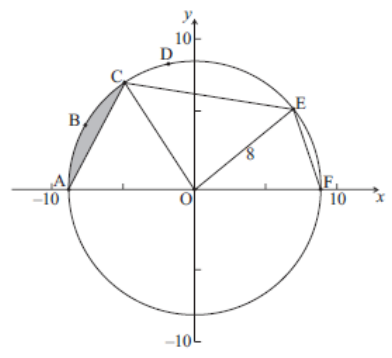
\includegraphics[scale=0.5]{figure_x9}\par
    \noindent Figure A.\par
  \end{center} % or flushleft or flushright
  \medskip
  \begin{center} % or flushleft or flushright
    \noindent Tableau de hauteurs de $P$ en mètres par rapport au sol après $t$ minutes.\par
    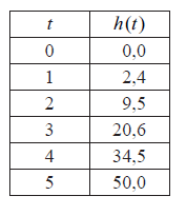
\includegraphics[scale=0.5]{tableau_x9}\par
    \noindent Tableau B.\par
  \end{center} % or flushleft or flushright

  \noindent Soit P un point de la roue. La roue démarre avec P à son point le plus bas, au niveau
du sol. La roue tourne avec une vitesse constante, dans le sens contraire des aiguilles
d’une montre. Un tour complet prend 20 minutes..\par
  \begin{enumerate}[label=(\alph*)]
  \item Donnez la hauteur de P par rapport au sol après
      \begin{enumerate}[label=(\roman*)]
        \item 10 minutes;
        \item 15 minutes.\hspace*{\fill} [2]
      \end{enumerate}
    \item Soit $h(t)$ la hauteur de $P$ par rapport au sol en mètres après $t$ minutes.
      \begin{enumerate}[label=(\roman*)]
        \item Montrez que $h(8)=90,5$
        \item Trouvez $h(21)$.\hspace*{\fill} [4]
      \end{enumerate}
    \item Esquissez la représentation graphique de $h$, avec $0 \le t \le 40.$\hspace*{\fill} [3]
    \item Étant donné que $h$ peut s’exprimer sous la forme $h(t) = a\,cos\,bt + c$, trouvez $a$ , $b$ et $c$.\hspace*{\fill} [5]
  \end{enumerate}
\end{question}
